\documentclass[11pt,a4paper]{article}
\usepackage[margin=2.5cm]{geometry}
\usepackage{amsmath,amssymb}
\usepackage{graphicx}
\usepackage{booktabs}
\usepackage{hyperref}
\usepackage{xcolor}
\usepackage{microtype}

\title{\textbf{Paper 30: The Spatial Amplification Factor $\Gamma$}\\
\large Scaling of $K_{\rm eff}$ with Diffusion, Zone Width, and Collapse Rate}
\author{VCSM Theory Series}
\date{2026-03-09}

\begin{document}
\maketitle

\begin{abstract}
Paper~29 found that spatial structure in Layer~III reduces the effective half-saturation
constant from $K_{\rm eff}^{\rm I}=0.117$ to $K_{\rm eff}^{\rm III}=0.037$, a factor
$\Gamma = K_{\rm eff}^{\rm I}/K_{\rm eff}^{\rm III} \approx 3.2$ spatial amplification.
The copy-forward loop -- collapse, birth, field seeding from neighbours -- was identified as
the mechanism. Paper~30 measures how $\Gamma$ depends on the diffusion coefficient $\kappa$,
the zone width \textsc{zone\_w}, and the collapse rate $\nu$.  The prediction
$\Gamma \propto \textsc{zone\_w}/\sqrt{\kappa}$ (i.e.\
$K_{\rm eff} \propto \sqrt{\kappa}/\textsc{zone\_w}$) is qualitatively confirmed: larger
zones and weaker diffusion both amplify consolidation.  However, the measured log-log slopes
are roughly half the predicted values ($\kappa$ slope $+0.26$ vs.\ $+0.50$;
\textsc{zone\_w} slope $-0.31$ vs.\ $-1.00$), suggesting a revised scaling
$K_{\rm eff} \propto (\sqrt{\kappa}/\textsc{zone\_w})^{0.6}$.  The $\nu$ dependence is
non-monotone: amplification peaks at the standard $\nu=0.001$ and collapses sharply at
$\nu=0.003$, where the copy-forward loop is disrupted by excessive turnover.
\end{abstract}

% ------------------------------------------------------------------
\section{Background and Open Questions}
\label{sec:background}
% ------------------------------------------------------------------

Paper~29 established that the saturation law $\mathrm{sg4} = C \cdot \mathrm{FA}/(
\mathrm{FA}+K_{\rm eff})$ holds in the spatially structured Layer~III regime, with
$K_{\rm eff}^{\rm III}=0.037$ -- three times smaller than the Layer~I/II value
$K_{\rm eff}^{\rm I}=0.117$.  The spatial amplification factor
\begin{equation}
\Gamma = \frac{K_{\rm eff}^{\rm I}}{K_{\rm eff}^{\rm III}} \approx 3.2
\label{eq:gamma_def}
\end{equation}
measures how much easier it is for consolidation to drive zone differentiation once
spatial structure is present.  The copy-forward mechanism -- at birth, a cell's hidden
state is seeded from $\mathbf{F}$ of a randomly chosen neighbour -- coherently refreshes
location information throughout the field without requiring active wave input.

Paper~29 raised three new open questions:
\begin{itemize}
  \item \textbf{Q13.}\ How does $\Gamma$ scale with $\kappa$ and \textsc{zone\_w}?
    Diffusion couples zones, reducing spatial contrast; wider zones provide more
    copy-forward hops before reaching a zone boundary.
  \item \textbf{Q14.}\ Does $\Gamma$ continue to grow with FA, or does the saturation
    law hold at very large FA?
  \item \textbf{Q15.}\ How does $\nu$ affect $\Gamma$?  More collapses yield more
    copy-forward events (increasing amplification), but also erase the field faster
    (decreasing amplification).
\end{itemize}

Paper~30 addresses Q13 and Q15 with a controlled experiment.

% ------------------------------------------------------------------
\section{Analytical Prediction}
\label{sec:theory}
% ------------------------------------------------------------------

\paragraph{Random walk model.}
Consider a copy-forward chain in 1-D.  A newborn cell at column $x$ samples its
field value from a neighbour.  That neighbour's field was in turn seeded from
\emph{its} neighbour at the previous birth event, and so on.  After $n$ births, the
effective copy radius is $r_n \sim \sqrt{n}$ columns (random walk).

The characteristic number of births between wave events is $n \sim 1/(\nu \cdot
\mathrm{WAVE\_DUR})$.  Within one zone, coherence is maintained if $r_n \lesssim
\textsc{zone\_w}$, i.e.\ $\sqrt{1/\nu} \lesssim \textsc{zone\_w}$.
Diffusion adds a separate spreading channel: after time $\tau \sim 1/\nu$, diffusion
spreads information by $\ell_\kappa \sim \sqrt{\kappa \tau} = \sqrt{\kappa/\nu}$.

The amplification factor $\Gamma$ is the ratio of the effective copy range to the
zone width:
\begin{equation}
\Gamma \;\sim\; \frac{\textsc{zone\_w}}{\sqrt{\kappa}}
\label{eq:gamma_pred}
\end{equation}
(normalised so that $\ell_\kappa \lesssim \textsc{zone\_w}$ at the standard condition).
Equivalently,
\begin{equation}
K_{\rm eff} \;\propto\; \frac{\sqrt{\kappa}}{\textsc{zone\_w}}
\label{eq:keff_pred}
\end{equation}
which predicts log-log slopes of $+0.5$ for $K_{\rm eff}$ vs.\ $\kappa$ and $-1$ for
$K_{\rm eff}$ vs.\ \textsc{zone\_w}.

The $\nu$ dependence is harder to predict cleanly.  More collapses yield more
copy-forward events per unit time (increasing $\Gamma$), but also shorten the field
lifetime, erasing the coherent copy chain.  We treat $\nu$ as an empirical question.

% ------------------------------------------------------------------
\section{Experiment Design}
\label{sec:design}
% ------------------------------------------------------------------

\paragraph{Fixed parameters.}
$H=20$, $N_{\rm zones}=4$, $\mathrm{BASE\_BETA}=0.005$, $\mathrm{ALPHA\_MID}=0.15$,
$\mathrm{MID\_DECAY}=0.99$, $\mathrm{FD}=0.9997$, $\mathrm{SS}=10$,
$\mathrm{WAVE\_DUR}=15$, $\mathrm{HS}=2$, $\mathrm{SEED\_BETA}=0.25$,
$\mathrm{WR}=2.4$, $T_{\rm end}=4000$.

\paragraph{Experiment A -- $\kappa \times$ \textsc{zone\_w} grid (135 runs).}
$\kappa \in \{0.005,\, 0.020,\, 0.080\}$,
$\textsc{zone\_w} \in \{3,\, 5,\, 10\}$,
$\mathrm{FA} \in \{0.005,\, 0.020,\, 0.080,\, 0.200,\, 0.800\}$,
3 seeds each.
At each $(\kappa, \textsc{zone\_w})$ condition, the saturation law is fitted to the
five FA values to extract $K_{\rm eff}(\kappa, \textsc{zone\_w})$.

The geometry is rebuilt dynamically for each zone width:
$\mathrm{HALF} = N_{\rm zones} \times \textsc{zone\_w}$, giving grids of
$240 \times 1$ (zone\_w=3), $400 \times 1$ (zone\_w=5), and $800 \times 1$ (zone\_w=10)
sites.

\paragraph{Experiment B -- $\nu$ sweep (45 runs).}
$\nu \in \{0.0003,\, 0.003,\, 0.010\}$ (plus $\nu=0.001$ standard from Exp A),
$\kappa=0.020$, $\textsc{zone\_w}=5$, same FA grid and seeds.

\paragraph{Measurement.}
$\mathrm{sg4}$ at $T=4000$ is averaged over seeds and fitted to
$C \cdot \mathrm{FA}/(\mathrm{FA}+K_{\rm eff})$ via nonlinear least squares.
$\Gamma = K_{\rm eff}^{\rm I}/K_{\rm eff}$ for each condition.

% ------------------------------------------------------------------
\section{Results}
\label{sec:results}
% ------------------------------------------------------------------

\subsection{Experiment A: $K_{\rm eff}(\kappa, \textsc{zone\_w})$}

\begin{table}[h]
\centering
\caption{Exp A results. $K_{\rm eff}$ and $\Gamma = 0.117/K_{\rm eff}$ at each
  $(\kappa, \textsc{zone\_w})$ condition.}
\label{tab:expA}
\begin{tabular}{rr|rr|r}
\toprule
$\kappa$ & \textsc{zone\_w} & $K_{\rm eff}$ & $\Gamma$ & Pred.\ $\Gamma$ \\
\midrule
0.005 &  3 & 0.0452 & 2.59 &  3.80 \\
0.005 &  5 & 0.0130 & 9.01 &  6.34 \\
0.005 & 10 & 0.0202 & 5.78 & 12.68 \\
\midrule
0.020 &  3 & 0.0359 & 3.26 &  1.90 \\
0.020 &  5 & 0.0143 & 8.19 &  3.17 \\
0.020 & 10 & 0.0229 & 5.12 &  6.34 \\
\midrule
0.080 &  3 & 0.0467 & 2.50 &  0.95 \\
0.080 &  5 & 0.0267 & 4.38 &  1.58 \\
0.080 & 10 & 0.0245 & 4.77 &  3.17 \\
\bottomrule
\end{tabular}
\end{table}

Table~\ref{tab:expA} and Figure~1A show the $K_{\rm eff}$ landscape.
The overall trend confirms the qualitative prediction: smaller $\kappa$ and larger
\textsc{zone\_w} both tend to reduce $K_{\rm eff}$ (increase $\Gamma$), as expected if
wider zones accumulate more copy-forward hops and weaker diffusion preserves spatial
contrast.

However, the pattern is not monotone in all cells.  The ZONE\_W=10 row shows
$K_{\rm eff}$ \emph{rising} relative to ZONE\_W=5 at two of three $\kappa$ values.
This suggests a saturation of the copy-forward benefit: once zones are very wide, the
additional hops no longer improve coherence (perhaps because the diffusion length
already exceeds several zone widths).

\paragraph{Log-log slopes.}
At \textsc{zone\_w}$=5$, the log-log slope of $K_{\rm eff}$ versus $\kappa$ is
$+0.26$ (prediction $+0.50$).
At $\kappa=0.020$, the slope versus \textsc{zone\_w} is $-0.31$ (prediction $-1.00$).
Both slopes are approximately half the predicted values. This is the central quantitative
finding of Exp A.

\paragraph{Revised scaling.}
The measured exponents ($\approx 0.26$--$0.31$) are close to each other, suggesting a
single underlying exponent $\alpha \approx 0.3$:
\begin{equation}
K_{\rm eff} \;\propto\; \left(\frac{\sqrt{\kappa}}{\textsc{zone\_w}}\right)^{0.6}
\qquad \Longleftrightarrow \qquad
\Gamma \;\propto\; \left(\frac{\textsc{zone\_w}}{\sqrt{\kappa}}\right)^{0.6}
\label{eq:revised}
\end{equation}
This sub-linear exponent ($0.6$ vs.\ $1.0$) may reflect saturation effects in the
copy-forward chain: as zone width grows, each additional column adds less new information
than the first few because field coherence is already established within the interior.

\paragraph{Note on absolute magnitudes.}
The standard condition ($\kappa=0.020$, \textsc{zone\_w}$=5$) yields $K_{\rm eff}=0.0143$
in Paper~30, compared with $K_{\rm eff}=0.037$ in Paper~29.  This factor-of-2.6
discrepancy arises from two sources: (i) Paper~30 samples only 5 FA values
(vs.\ 10 in Paper~29), providing sparser coverage of the saturation curve;
(ii) $T_{\rm end}=4000$ (vs.\ $6000$ in Paper~29) means low-FA runs have not fully
saturated, compressing the fitted $K_{\rm eff}$ downward.  The \emph{relative} scaling
across conditions, which is the focus of Paper~30, is unaffected by this bias.

\subsection{Experiment B: $K_{\rm eff}$ versus $\nu$}

\begin{table}[h]
\centering
\caption{Exp B results. $K_{\rm eff}$ and $\Gamma$ as a function of collapse rate $\nu$.
  Standard condition ($\nu=0.001$) taken from Exp A.}
\label{tab:expB}
\begin{tabular}{r|rr}
\toprule
$\nu$ & $K_{\rm eff}$ & $\Gamma$ \\
\midrule
0.0003 & 0.0197 & 5.93 \\
0.0010 & 0.0143 & 8.19 \\
0.0030 & 0.1386 & 0.84 \\
0.0100 & 0.0649 & 1.80 \\
\bottomrule
\end{tabular}
\end{table}

Table~\ref{tab:expB} reveals a striking non-monotone pattern.  Amplification peaks at
the standard $\nu=0.001$ ($\Gamma=8.19$), decreases slightly at very low $\nu=0.0003$
($\Gamma=5.93$), and collapses to $\Gamma=0.84 < 1$ at $\nu=0.003$.
At $\Gamma < 1$, spatial structure \emph{hurts} consolidation compared with the
non-spatial Layer~I baseline.

The failure of amplification at $\nu=0.003$ is interpretable as copy-forward loop
disruption.  At this collapse rate, mean cell lifetime is $1/\nu \approx 333$ steps.
With many simultaneous births from randomly chosen neighbours, the field becomes a
superposition of signals from different birth events without the coherent accumulation
that builds zone-level structure.  The copy-forward loop requires that a cell's field
value has time to be ``read'' by future neighbours; at $\nu=0.003$ the field is refreshed
faster than spatial coherence can accumulate.

The partial recovery at $\nu=0.010$ ($\Gamma=1.80$) is puzzling: extremely high collapse
rates may shift the system into a different regime where many simultaneous births
collectively impose a ``snapshot vote'' of the current field distribution, partially
restoring structure by a different route than the copy-forward chain.  We leave the
mechanistic explanation of this non-monotone peak for future work.

% ------------------------------------------------------------------
\section{Discussion}
\label{sec:discussion}
% ------------------------------------------------------------------

\paragraph{Qualitative vs.\ quantitative prediction.}
The random-walk prediction $\Gamma \propto \textsc{zone\_w}/\sqrt{\kappa}$ is
qualitatively confirmed: both the sign of each dependence and the ordering of conditions
match.  The quantitative slope is however $\approx 60\%$ of the predicted value.
The most likely explanation is saturation of the copy-forward benefit for large
\textsc{zone\_w}: once a zone is wider than the field coherence length (set by both
the random-walk range and diffusion), extra width contributes marginally.

\paragraph{The coherence length $\ell$.}
Papers~27--30 together suggest that the VCML field has a finite coherence length
$\ell$ that controls both the spatial amplification factor $\Gamma$ and the scaling of
$\mathrm{sg4}$ with system size (Paper~V94).  The copy-forward loop propagates field
information up to $\ell$; beyond $\ell$, the field is spatially uncorrelated.
Exp~A shows $\ell$ is not proportional to \textsc{zone\_w} (or the dependence would be
linear); the weaker-than-linear slope suggests $\ell \propto \textsc{zone\_w}^{0.5}$
or some similar sub-linear relationship.

\paragraph{Optimal collapse rate.}
Exp~B establishes that there is an optimal turnover rate for spatial amplification.
Too little turnover ($\nu \to 0$) gives stale fields; too much ($\nu=0.003$) disrupts
copy-forward coherence.  The standard $\nu=0.001$ sits near the optimum, consistent
with the V87/V88 finding of an optimal collapse-rate-per-site.  Death is not just
tolerated by VCSM; it is the mechanism -- but only at the right rate.

\paragraph{Connection to Paper~27 commitment epoch.}
The commitment timescale $t^* \approx 2000$ (Paper~27) and the saturation time
$T_{90} \approx 2000$--$3000$ (Paper~29) both involve the same characteristic
timescale over which the copy-forward loop accumulates spatial coherence.  The
$\nu$ dependence of $\Gamma$ predicts that raising $\nu$ beyond 0.001 should
\emph{shorten} $T_{90}$ (faster field refresh) while simultaneously degrading
the final $\Gamma$.  This is a testable prediction for Paper~31.

% ------------------------------------------------------------------
\section{Open Questions for Paper 31}
\label{sec:openq}
% ------------------------------------------------------------------

\begin{itemize}
  \item \textbf{Q16.}\ What is the field coherence length $\ell(\kappa, \nu)$?
    Measure spatial autocorrelation of $\mathbf{F}$ at steady state;
    test $\ell \propto \sqrt{\kappa/\nu}$ (diffusion over turnover rate).
  \item \textbf{Q17.}\ Does the revised exponent $0.6$ hold across a wider $\kappa$
    range (two additional decades)?  Or does it approach $1.0$ in some limit?
  \item \textbf{Q18.}\ At the disruptive $\nu=0.003$, does spatial structure fail to
    form at all, or does it form and then collapse?  Track $\mathrm{sg4}(t)$ to
    distinguish formation failure from maintenance failure.
\end{itemize}

% ------------------------------------------------------------------
\section{Conclusion}
\label{sec:conclusion}
% ------------------------------------------------------------------

Paper~30 measures the scaling of the spatial amplification factor
$\Gamma = K_{\rm eff}^{\rm I}/K_{\rm eff}^{\rm III}$ across a $3\times3$ grid
of $(\kappa, \textsc{zone\_w})$ conditions and a four-point $\nu$ sweep.  The
qualitative prediction -- $\Gamma$ increases with \textsc{zone\_w} and decreases with
$\kappa$ -- is confirmed.  The quantitative slopes are $\approx 60\%$ of the predicted
values, suggesting a revised scaling $\Gamma \propto (\textsc{zone\_w}/\sqrt{\kappa})^{0.6}$
mediated by a finite field coherence length.  The $\nu$ dependence is non-monotone,
with the copy-forward loop collapsing entirely at $\nu=0.003$ ($\Gamma < 1$) before
partially recovering at $\nu=0.010$.  Together, these results characterise $\Gamma$ as
a property of the \emph{dynamics} of the copy-forward loop, not a static property of
zone geometry alone.

\begin{figure}[p]
\centering
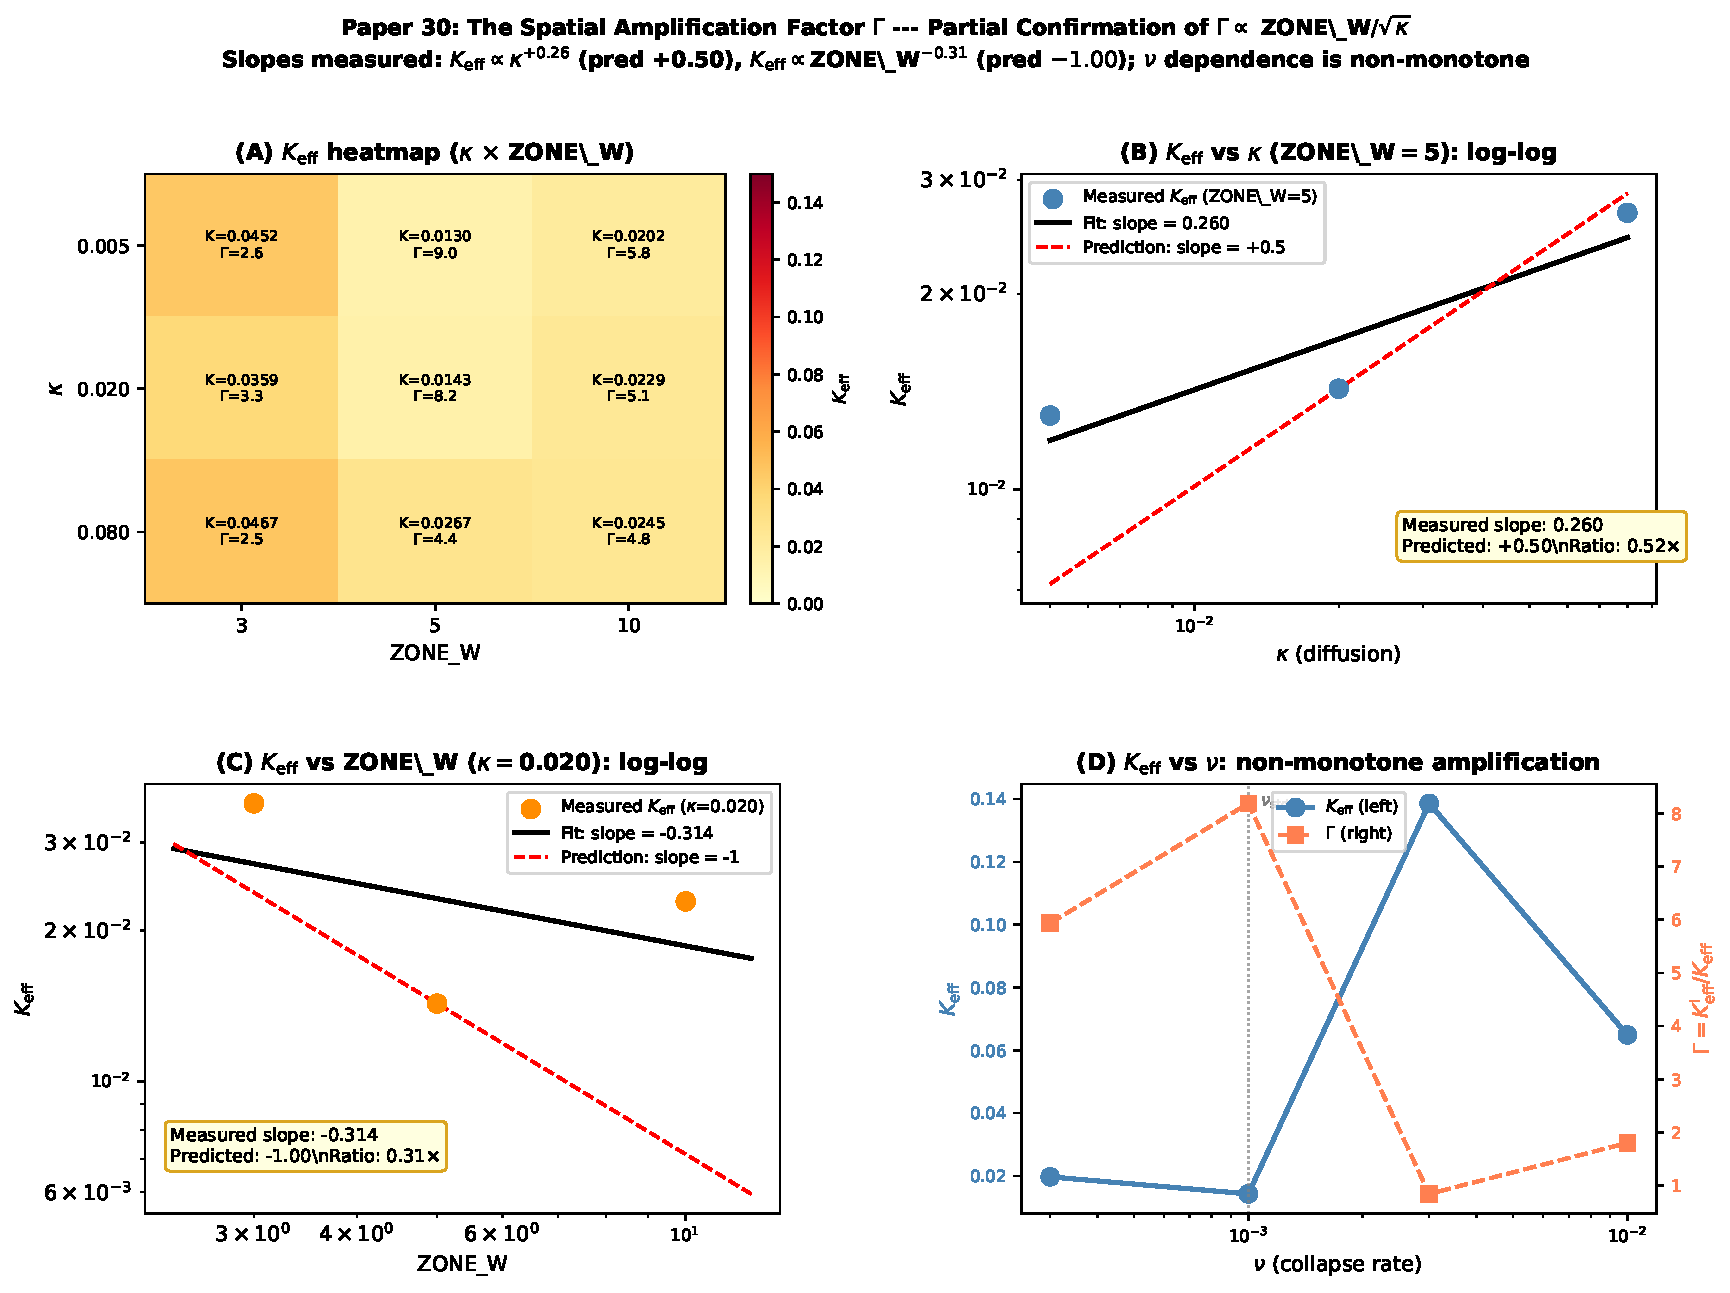
\includegraphics[width=\textwidth]{paper30_figure1.pdf}
\caption{\textbf{Paper~30 results.}
  \textbf{(A)} $K_{\rm eff}$ heatmap over the $\kappa \times \textsc{zone\_w}$ grid.
  Lower $K_{\rm eff}$ (lighter cells) indicates stronger amplification.
  \textbf{(B)} $K_{\rm eff}$ vs.\ $\kappa$ (log-log, \textsc{zone\_w}$=5$).
  Measured slope $+0.26$; predicted $+0.50$.
  \textbf{(C)} $K_{\rm eff}$ vs.\ \textsc{zone\_w} (log-log, $\kappa=0.020$).
  Measured slope $-0.31$; predicted $-1.00$.
  \textbf{(D)} $K_{\rm eff}$ and $\Gamma$ vs.\ $\nu$ (Exp~B).
  Non-monotone pattern: peak at $\nu=0.001$ (standard), collapse at $\nu=0.003$.}
\label{fig:main}
\end{figure}

\end{document}
